% This file was created with tikzplotlib v0.10.1.
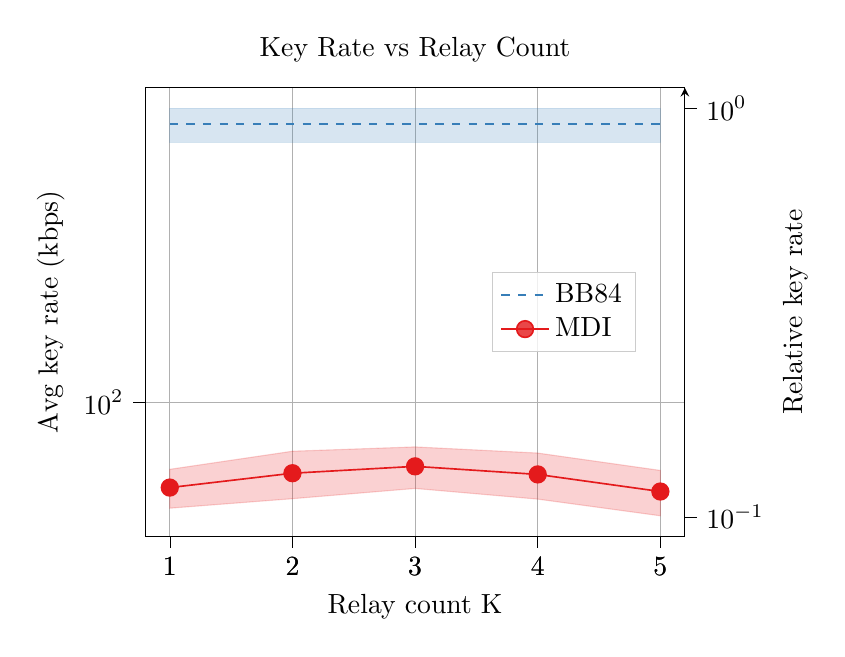
\begin{tikzpicture}

\definecolor{crimson2282628}{RGB}{228,26,28}
\definecolor{darkgray176}{RGB}{176,176,176}
\definecolor{darkorange25512714}{RGB}{255,127,14}
\definecolor{lightgray204}{RGB}{204,204,204}
\definecolor{steelblue31119180}{RGB}{31,119,180}
\definecolor{steelblue55126184}{RGB}{55,126,184}

\begin{axis}[
legend cell align={left},
legend style={
  fill opacity=0.8,
  draw opacity=1,
  text opacity=1,
  at={(0.91,0.5)},
  anchor=east,
  draw=lightgray204
},
log basis y={10},
tick align=outside,
tick pos=left,
x grid style={darkgray176},
xlabel={Relay count K},
xmajorgrids,
xmin=0.8, xmax=5.2,
xtick style={color=black},
xtick={1,2,3,4,5},
xticklabels={
  \(\displaystyle {1}\),
  \(\displaystyle {2}\),
  \(\displaystyle {3}\),
  \(\displaystyle {4}\),
  \(\displaystyle {5}\)
},
y grid style={darkgray176},
ylabel={Avg key rate (kbps)},
ymajorgrids,
ymin=43.2625132575724, ymax=714.577526943153,
ymode=log,
ytick style={color=black},
ytick={1,10,100,1000,10000},
yticklabels={
  \(\displaystyle {10^{0}}\),
  \(\displaystyle {10^{1}}\),
  \(\displaystyle {10^{2}}\),
  \(\displaystyle {10^{3}}\),
  \(\displaystyle {10^{4}}\)
}
]
\path [draw=steelblue55126184, fill=steelblue55126184, opacity=0.2]
(axis cs:1,629.054905453169)
--(axis cs:1,508.741806872021)
--(axis cs:2,508.741806872021)
--(axis cs:3,508.741806872021)
--(axis cs:4,508.741806872021)
--(axis cs:5,508.741806872021)
--(axis cs:5,629.054905453169)
--(axis cs:5,629.054905453169)
--(axis cs:4,629.054905453169)
--(axis cs:3,629.054905453169)
--(axis cs:2,629.054905453169)
--(axis cs:1,629.054905453169)
--cycle;

\path [draw=crimson2282628, fill=crimson2282628, opacity=0.2]
(axis cs:1,65.7261474772101)
--(axis cs:1,51.5425769884114)
--(axis cs:2,54.6941225650712)
--(axis cs:3,58.3203331791175)
--(axis cs:4,54.5544176339571)
--(axis cs:5,49.1442312347454)
--(axis cs:5,65.2686892884814)
--(axis cs:5,65.2686892884814)
--(axis cs:4,72.7736445964739)
--(axis cs:3,75.6157843520762)
--(axis cs:2,73.5995778695195)
--(axis cs:1,65.7261474772101)
--cycle;

\addplot [semithick, steelblue55126184, dashed]
table {%
1 568.898356162595
2 568.898356162595
3 568.898356162595
4 568.898356162595
5 568.898356162595
};
\addlegendentry{BB84}
\addplot [semithick, crimson2282628, mark=*, mark size=3, mark options={solid}]
table {%
1 58.6343622328107
2 64.1468502172953
3 66.9680587655969
4 63.6640311152155
5 57.2064602616134
};
\addlegendentry{MDI}
\end{axis}

\begin{axis}[
axis y line=right,
log basis y={10},
tick align=outside,
title={Key Rate vs Relay Count},
x grid style={darkgray176},
xmin=0.8, xmax=5.2,
xtick pos=left,
xtick style={color=black},
y grid style={darkgray176},
ylabel={Relative key rate},
ymin=0.0896460001657405, ymax=1.12170712928006,
ymode=log,
ytick pos=right,
ytick style={color=black},
ytick={0.001,0.01,0.1,1,10,100},
yticklabel style={anchor=west},
yticklabels={
  \(\displaystyle {10^{-3}}\),
  \(\displaystyle {10^{-2}}\),
  \(\displaystyle {10^{-1}}\),
  \(\displaystyle {10^{0}}\),
  \(\displaystyle {10^{1}}\),
  \(\displaystyle {10^{2}}\)
}
]
\addplot [semithick, steelblue31119180, opacity=0]
table {%
1 1
2 1
3 1
4 1
5 1
};
\addplot [semithick, darkorange25512714, opacity=0]
table {%
1 0.103066499661413
2 0.112756258692654
3 0.117715331816598
4 0.111907567363439
5 0.100556557497353
};
\end{axis}

\end{tikzpicture}
